%% DASH manuscript prepared for the Journal of Systems and Software
%% Elsevier CAS double-column template (cas-dc)
%% Revision v4 (2026-10-11): restructured around the Controlled Replication
%% and Mechanism Study; see change_log.txt and claim_evidence_ledger.csv.
\documentclass[a4paper,fleqn]{cas-dc}
\usepackage[authoryear]{natbib}
\usepackage{amsthm}
\newtheorem{proposition}{Proposition}
\usepackage{array}
\usepackage{multirow}
\usepackage{placeins}
\usepackage{tabularx}
\usepackage{xurl}
\usepackage{tikz}
\usetikzlibrary{arrows.meta,positioning,fit,backgrounds,shapes.geometric}
\usepackage{adjustbox}
\graphicspath{{figures/}}
\newcolumntype{Y}{>{\raggedright\arraybackslash}X}

\begin{document}
\let\WriteBookmarks\relax
\def\floatpagepagefraction{1}
\def\textpagefraction{.001}

\shorttitle{DASH: Bounded-state execution for streaming ML}
\shortauthors{S. Kim and V. L. R. Chinthalapati}

\title [mode = title]{DASH: Bounded-State Execution for Low-Latency Streaming Machine Learning with Externalised State}

\author[1]{Seonwoo Kim}[orcid=0009-0005-9599-0514]
\ead{skim008@gold.ac.uk}
\credit{Conceptualization, Methodology, Software, Validation, Formal analysis, Investigation, Data curation, Visualization, Writing -- original draft, Writing -- review \& editing}

\author[1]{V. L. Raju Chinthalapati}
\cormark[1]
\ead{v.chinthalapati@gold.ac.uk}
\credit{Conceptualization, Methodology, Supervision, Project administration, Formal analysis, Validation, Writing -- review \& editing}

\affiliation[1]{organization={School of Computing, Goldsmiths, University of London},
            addressline={New Cross},
            city={London},
            postcode={SE14 6NW},
            country={United Kingdom}}

\cortext[1]{Corresponding author}

\begin{abstract}
Streaming machine-learning services often keep per-stream state in an external store so that it can be shared, inspected or recovered, while decisions must meet tight latency budgets. A common implementation reads the recent feature window back before every prediction, even when the model uses only the current vector. DASH is a bounded-state design that maintains a fixed-length window per stream with one atomic update, feeds current-vector classifiers without reading the window back, invokes a second-stage model conditionally, and keeps durable storage off the synchronous path. In a controlled replication on two heterogeneous single-host environments, the bounded path (A) and a window-fetching path (B1) share writer, layout, models and schedule, and agree on every predicted label checked. B1's state-access time grows with window length $W$ while A's stays nearly flat, and the Redis key footprint is constant in history length $N$ for fixed $W$. Median latency is lower for A in every paired repeat; the P99 advantage holds in both environments with 100 resident streams but reverses in one environment with a single stream. A breadth evaluation of three model families on both environment types and a third host again lowered median latency in every repeat; on the original input, tail gains held for logistic regression and XGBoost where not flagged as noisy, but were inconsistent for random forest. The benefit is reduced external-state access cost, not a universal tail-latency guarantee.
\end{abstract}

\begin{highlights}
\item Window fetching adds state cost that grows with window length; the update stays flat.
\item Per-stream Redis window state is constant in stream length for a fixed window.
\item Median latency is lower without the window read in every paired repeat.
\item The P99 direction holds with 100 streams but reverses in one single-stream cell.
\item External state is a requirement; its durability is configured, not measured.
\end{highlights}

\begin{keywords}
streaming machine learning \sep externalised state \sep software architecture for ML systems \sep bounded state \sep tail latency \sep performance evaluation
\end{keywords}

\maketitle

%% ==================================================================
\section{Introduction}
\label{sec:intro}
%% ==================================================================
A machine-learning model that runs over a continuous event stream is one component of a larger software system. Before each decision, the system must update per-stream state, assemble the model input and invoke one or more models, and it must often make that state available to other components. Requirements such as sharing state between processes, inspecting it from outside the inference process, separating inference from storage, and restoring it after a restart are frequently met by placing state in an external store. Each of these requirements adds work to the synchronous decision path, and the way the state is accessed determines how much.

A recurring implementation pattern keeps a recent window of feature vectors in an external store and reads the whole window back before every prediction. The pattern is simple and general, but when the model consumes only the current feature vector the read is unnecessary: it adds a transfer, deserialisation and materialisation step whose size grows with the window length $W$. Keeping all state in local process memory avoids this cost but gives up the properties that motivated externalisation. The design question is therefore not whether external state is faster than local memory, but how much synchronous cost a given state-access discipline imposes once external state is required.

We study this question through DASH, a bounded-state execution design. DASH maintains a fixed-length per-stream window in Redis through a single atomic server-side update, supplies current-vector classifiers with the current vector without reading the window back, invokes a second-stage model only when a first-stage gate opens, and writes durable history asynchronously. The application workload is market-shock screening on one-second cryptocurrency trade aggregates; the predictive models are fixed artefacts that generate realistic inference work, not contributions in their own right.

The evaluation compares three execution paths that use the same models, inputs and request schedule: the bounded path~A, a window-fetching path~B1 that uses the same writer and stored layout but additionally reads and decodes the window, and an in-process reference~B2 that does not access Redis. It is organised around three research questions.

\textbf{RQ1.} For current-vector streaming classifiers, does avoiding full-window retrieval reduce the execution cost of maintaining externally accessible state, and how consistent is the effect across execution environments?

\textbf{RQ2.} What mechanism explains the observed cost difference, and how does the bounded state depend on stream history and configured window length?

\textbf{RQ3.} Which architectural trade-offs and validity boundaries govern the use of the external-state execution path?


RQ1 and RQ2 are answered empirically. RQ3 is answered by combining the measurements with the requirements that motivate external state; it is not a recovery or fault-tolerance experiment.

The primary evidence is a \emph{Controlled Replication and Mechanism Study} of the final Lua-based implementation in two heterogeneous environments under rules fixed before measurement, complemented by a \emph{Breadth Evaluation} that applies the same implementation, artefacts and protocol to all three model families in both replication environment types with the original input and on a third host with a different data set. An evaluation of an earlier implementation is not used, because its trial-level records could not be matched to its reported protocol (Section~\ref{subsec:breadth}).

\paragraph{Contributions}
\begin{enumerate}
  \item An implementation-grounded bounded-state and access model that states the per-stream state and per-tick access cost of each execution path with explicit dependence on history length $N$, window length $W$ and number of resident streams $K$, and separates what the architecture bounds from what it does not (Section~\ref{sec:model}).
  \item A controlled replication and mechanism study in which the compared paths share writer, stored layout, models and schedule, with prediction-equivalence checks, window-length and memory experiments, and an explicit report of tail-latency reversals (Sections~\ref{sec:setup}--\ref{sec:results}).
  \item A reproducibility package with pinned code and artefact hashes and a requirements-based interpretation of when external rather than local state is justified (Sections~\ref{sec:discussion} and~\ref{sec:threats}).
\end{enumerate}
DASH is not a new classifier, a new stream-processing engine, or a claim that external state can outperform local memory.

Section~\ref{sec:related} positions the work. Section~\ref{sec:model} describes the workload, execution paths and access model. Section~\ref{sec:setup} gives the evaluation design and Section~\ref{sec:results} the results. Section~\ref{sec:discussion} discusses the architectural trade-offs (RQ3), Section~\ref{sec:threats} the threats to validity, and Section~\ref{sec:conclusion} concludes.

%% ==================================================================
\section{Related Work}
\label{sec:related}
%% ==================================================================
\subsection{Stateful Stream Processing and Window Maintenance}
Distributed stream processors such as Kafka, Storm, Spark Streaming and Flink provide durable logs, operator parallelism and managed state \citep{carbone2015flink,kreps2011kafka,toshniwal2014storm,zaharia2013discretized}. The Dataflow model relates correctness, latency and cost for unbounded data \citep{akidau2015dataflow}, sliding-window semantics directly determine the computation and memory of window operators \citep{golab2006sliding}, and making operator state explicit enables its management and recovery \citep{fernandez2015liquid}. Bounded window state is therefore not new. The question studied here is narrower: how much of that state must be materialised synchronously on each inference tick when the model consumes only the current feature vector. Table~\ref{tab:paradigms} makes the distinction explicit.

\begin{table}[pos=htbp]
  \centering
  \caption{State-access patterns. $W$ is a fixed window and $d$ the feature dimension; dependence on history length $N$ is per stream. External state and conditional inference are independent design choices.}
  \label{tab:paradigms}
  \small
  \begin{tabularx}{\linewidth}{@{}Y l l@{}}
    \toprule
    Pattern & Stored state & Per-tick read \\
    \midrule
    Full-history recomputation & $\mathcal{O}(Nd)$ & $\mathcal{O}(Nd)$ \\
    Fixed window, fetched each tick (B1) & $\mathcal{O}(Wd)$ & $\mathcal{O}(Wd)$ \\
    Fixed window, current vector only (A) & $\mathcal{O}(Wd)$ & $\mathcal{O}(d)$ \\
    Local recurrence, no external state & $\mathcal{O}(d)$ & local only \\
    \bottomrule
  \end{tabularx}
\end{table}

For fixed $W$ and $d$, both window rows are $\mathcal{O}(1)$ in $N$. DASH does not claim a different asymptotic class from a fixed-window store; it avoids the repeated transfer and materialisation of a window that a current-vector consumer does not need.

\subsection{ML Serving and the Separation of State}
Prediction-serving systems such as Clipper optimise model invocation but treat input features as already computed \citep{crankshaw2017clipper}, and feature stores separate the computation and serving of features from model execution \citep{delaruamartinez2024hopsworks}. Lakehouse architectures keep durable analytical data on object storage \citep{armbrust2020delta,zaharia2021lakehouse}. DASH follows the same separation of concerns at a smaller scale: a small hot tier serves the decision path and a cold tier holds history for retraining and audit. Its focus is the synchronous access discipline between the inference process and the hot tier, which these systems leave to the application.

\subsection{Operating Thresholds Under Imbalance and Drift}
Rare-event detectors are evaluated with precision--recall rather than ROC analysis because the positive class is small \citep{saito2015pr}, and their operating thresholds are usually chosen on validation data. In non-stationary streams, the score distribution and therefore the rate at which a fixed threshold fires can change over time \citep{gama2014drift}. For a gated pipeline this matters to systems evaluation as well as to accuracy: the gate rate determines how often the expensive stage runs, so latency measured at an unrepresentative threshold or on unrepresentative data can hide the downstream model. We therefore keep the stored thresholds fixed, measure the realised Stage-2 rate in every cell, and report it with the latency.

\subsection{Tail Latency, Conditional Inference and Benchmarking}
Small component delays are amplified into tail latency in large services \citep{dean2013tail}; operator placement \citep{ecker2025latency} and redundancy management \citep{shokhanda2025safetail} address the tail at deployment level. Early-exit and conditional execution reduce average compute by stopping when an early stage is confident \citep{passalis2020adaptive}; the two-stage gate in DASH plays this role but does not bound the latency of a request for which the gate opens. On the evaluation side, Linear Road introduced response-time-constrained stream benchmarking \citep{arasu2004linearroad}, Theodolite benchmarks scalability of stream processing microservices \citep{henning2023theodolite}, and recent work evaluates fault recovery through latency distributions rather than throughput alone \citep{vogel2024fault}. Following these, we report latency distributions per repeat rather than single summary values. Machine-learning methods for abnormal activity in cryptocurrency markets \citep{monamo2016bitcoin,gu2025fraud} motivate the workload but are not the subject of this paper.

%% ==================================================================
\section{System Model and Execution Paths}
\label{sec:model}
%% ==================================================================
\subsection{Requirements and Design Overview}
\label{subsec:design}
DASH targets services in which per-stream state must be readable outside the inference process (for example by alert consumers, audit tools or a restarted worker) and in which inference must remain fast. Redis is used as the hot tier because it offers low-latency list operations, server-side scripting, access from several processes, and optional persistence through snapshots or an append-only file \citep{redis2023}. These are \emph{requirements and capabilities}; whether a deployment actually obtains durability or recovery depends on its configuration and recovery protocol, which this paper does not evaluate. Figure~\ref{fig:arch} shows the conceptual pipeline and marks the boundary of the timed execution path.

\begin{figure*}[pos=htbp]
\centering
\begin{adjustbox}{max width=\linewidth}
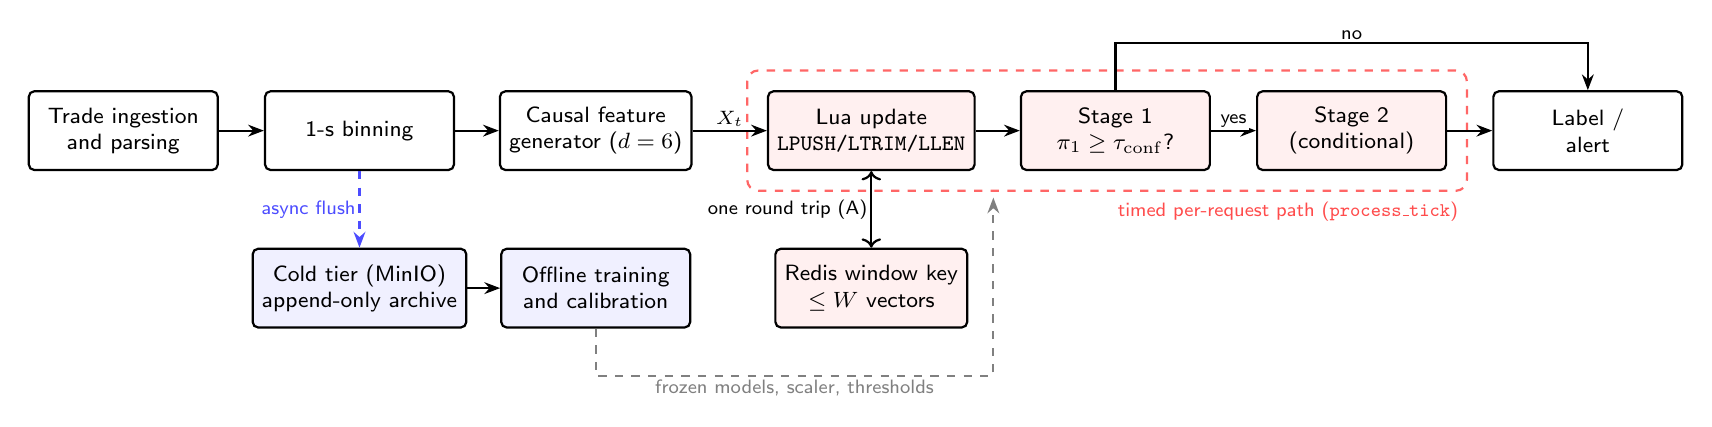
\begin{tikzpicture}[
  x=1mm, y=1mm,
  font=\footnotesize\sffamily,
  box/.style={draw, rounded corners=2pt, align=center, minimum width=24mm, minimum height=10mm, fill=white, thick},
  hot/.style={box, fill=red!6},
  cold/.style={box, fill=blue!6},
  arrow/.style={-{Stealth[length=2mm]}, thick},
  lab/.style={fill=white, inner sep=1pt, font=\scriptsize\sffamily}
]
\node[box] (ing) at (0,0) {Trade ingestion\\and parsing};
\node[box] (bin) at (30,0) {1-s binning};
\node[box] (feat) at (60,0) {Causal feature\\generator ($d=6$)};
\node[hot] (upd) at (95,0) {Lua update\\\texttt{LPUSH/LTRIM/LLEN}};
\node[hot] (s1) at (126,0) {Stage~1\\$\pi_1\ge\tau_{\mathrm{conf}}$?};
\node[hot] (s2) at (156,0) {Stage~2\\(conditional)};
\node[box] (out) at (186,0) {Label /\\alert};
\node[cold] (minio) at (30,-20) {Cold tier (MinIO)\\append-only archive};
\node[cold] (train) at (60,-20) {Offline training\\and calibration};
\node[hot] (redis) at (95,-20) {Redis window key\\$\le W$ vectors};
\draw[arrow] (ing) -- (bin);
\draw[arrow] (bin) -- (feat);
\draw[arrow] (feat) -- node[lab, above]{$X_t$} (upd);
\draw[arrow] (upd) -- (s1);
\draw[arrow] (s1) -- node[lab, above]{yes} (s2);
\draw[arrow] (s2) -- (out);
\draw[arrow] (s1.north) -- ++(0,6) -| node[lab, pos=0.25, above]{no} (out.north);
\draw[arrow, <->] (upd.south) -- node[lab, left]{one round trip (A)} (redis.north);
\draw[arrow, blue!70, dashed] (bin.south) -- node[lab, left]{async flush} (minio.north);
\draw[arrow] (minio) -- (train);
\draw[arrow, gray, dashed] (train.south) -- ++(0,-6) -| node[lab, pos=0.25, below]{frozen models, scaler, thresholds} (110.5,-8.5);
\begin{scope}[on background layer]
\node[draw=red!60, dashed, thick, rounded corners, inner sep=2.5mm, fit=(upd)(s1)(s2),
      label={[font=\scriptsize\sffamily, red!70, anchor=north east]south east:timed per-request path (\texttt{process\_tick})}] {};
\end{scope}
\end{tikzpicture}
\end{adjustbox}
\caption{DASH pipeline and measurement boundary. The timed path starts from a prepared feature vector and ends when the label is returned; ingestion, binning, feature generation, cold-tier writes and alert delivery are outside it. In B1 the same update is followed by an \texttt{LRANGE} read of the window; B2 replaces Redis with a local array (Table~\ref{tab:paths}).}
\label{fig:arch}
\end{figure*}

\subsection{Workload: Features, Labels and Two-Stage Decision}
\label{subsec:workload}
Table~\ref{tab:notation} lists the parameters used throughout.

\begin{table}[pos=htbp]
\caption{Notation and fixed parameters.}\label{tab:notation}
\small
\begin{tabularx}{\linewidth}{@{}l Y@{}}
\toprule
Symbol & Meaning \\
\midrule
$t$ & Index of populated one-second rows of a stream \\
$N$ & Rows processed for a stream (history length) \\
$K$ & Resident logical streams with independent state \\
$W$ & Length of the Redis feature window (default 30) \\
$d$ & Feature dimension ($d=6$, float32) \\
$W_{\mathrm{vol}}$ & Rolling volume-baseline length of the feature generator (60 rows), independent of $W$ \\
$H$ & Label horizon in populated rows ($H=30$) \\
$\alpha,\lambda$ & Label threshold multiplier (2.0) and EWMA decay (0.94) \\
$\tau_{\mathrm{conf}},\tau_{s2}$ & Stored Stage-1 gate and Stage-2 decision thresholds \\
A, B1, B2 & Bounded, window-fetching and in-process execution paths (Table~\ref{tab:paths}) \\
\bottomrule
\end{tabularx}
\end{table}

For each stream $k$, trades are aggregated into one-second bins; empty seconds produce no row, so $t$ indexes populated rows. The feature vector is
\begin{equation}
\label{eq:featurevec}
X_t^{(k)} = \bigl[r_t,\,\hat\sigma_t,\,\mathrm{OFI}_t,\,\mathrm{Imb}_t,\,\mathrm{VolSpike}_t,\,C_t\bigr]^{\top},
\end{equation}
in this order: the log return of the volume-weighted average price (VWAP) over the previous row, an EWMA volatility $\hat\sigma_t=\sqrt{v_t+\epsilon}$ with $v_t=\lambda v_{t-1}+(1-\lambda)r_t^2$ and $\lambda=0.94$, the buy-minus-sell aggressor volume $\mathrm{OFI}_t$, its normalised version $\mathrm{Imb}_t=\mathrm{OFI}_t/(Q_{t,\mathrm{buy}}+Q_{t,\mathrm{sell}}+\epsilon)$, the ratio of current volume to a rolling mean over the last $W_{\mathrm{vol}}=60$ populated rows, and the trade count. All features are causal: they use rows up to and including $t$. Order-flow imbalance, defined by \citet{cont2011price} from order-book events and approximated here by signed trade volume, and trading volume are standard short-horizon microstructure signals. $W_{\mathrm{vol}}$ belongs to the feature generator and is unrelated to the Redis window length $W$; with $W_{\mathrm{vol}}$ fixed, the generator's per-row cost is bounded. Full definitions are given in Supplement~S1.

The offline label uses the forward return over the next $H=30$ populated rows, $R^{(H)}_t=\sum_{i=1}^{H} r_{t+i}$, and assigns $y_t=2$ (positive shock) if $R^{(H)}_t\ge\alpha\sqrt{H}\hat\sigma_t$, $y_t=1$ (negative shock) if $R^{(H)}_t\le-\alpha\sqrt{H}\hat\sigma_t$, and $y_t=0$ otherwise, with $\alpha=2$. Because $H$ counts populated rows, it equals 30~s only when no second is empty. The last $H$ rows have no label and are dropped. The labels are an operational proxy for abnormal short-horizon movements, not evidence of manipulation.

Stage~1 estimates $\pi_{1,t}=f_1(X_t)\approx\mathbb{P}(y_t\in\{1,2\}\mid X_t)$. If $\pi_{1,t}\ge\tau_{\mathrm{conf}}$, Stage~2 estimates $\pi_{2,t}=f_2(X_t)$, the probability of a positive shock given a shock, and the output is $\hat y_t=2$ if $\pi_{2,t}\ge\tau_{s2}$ and $\hat y_t=1$ otherwise; if the gate does not open, $\hat y_t=0$. The gate is a compute-admission rule: it changes how often the Stage-2 model runs, not the dependence of per-tick work on $N$.

\subsection{Execution Paths}
\label{subsec:paths}
Table~\ref{tab:paths} specifies the three paths as implemented at the pinned commit. A and B1 call the same writer, a Lua script that pushes the new float32 vector, trims the list to $W$ entries and returns its length in one atomic server-side step. A then passes the current vector to the models. B1 additionally reads the window with \texttt{LRANGE}, decodes up to $W$ vectors, stacks them, and passes the last (current) vector to the same models. A and B1 therefore store the same state and use the same model input; they differ only in the read and materialisation step. B2 holds the replay array in process memory, slices the last $W$ rows, computes z-scores and differences over the slice to represent window-dependent work, discards the result, and passes the current vector to the models.

\begin{table*}[pos=htbp]
\caption{Execution paths compared. All three use the same frozen model, scaler and threshold artefacts and the same request schedule within a repeat. ``Measured'' refers to the quantities reported in Section~\ref{sec:results}; ``not measured'' lists operational properties that motivate the design but were not evaluated.}
\label{tab:paths}
\small
\begin{tabularx}{\linewidth}{@{}>{\raggedright\arraybackslash}p{0.11\linewidth}YYYY>{\raggedright\arraybackslash}p{0.13\linewidth}Y@{}}
\toprule
Path & State placement & Synchronous state operations per tick & Model input & Stored footprint per stream & Measured & Not measured \\
\midrule
A (DASH) & External Redis list, $\le W$ float32 vectors & One Lua call: \texttt{LPUSH}, \texttt{LTRIM}, \texttt{LLEN} & Current vector & $\mathcal{O}(Wd)$; constant in $N$ & Latency, state interval, key memory & Durability, failover, multi-writer correctness \\
B1 (window fetch) & Same key and layout as A & Same Lua call, then \texttt{LRANGE} and decoding of up to $W$ vectors & Current vector, selected from the decoded window & Identical to A & Latency, state interval & As for A \\
B2 (in-process reference) & Local array in the inference process & None in Redis; slice of $W$ rows and z-score/difference computation & Current vector & Window slice of a replay array that may hold the whole input & Latency, state interval & Not externally accessible \\
\bottomrule
\end{tabularx}
\end{table*}

B1 is a deliberately window-fetching access-pattern baseline, not an optimised current-vector Redis client or a managed-state stream processor. B2 is an in-process reference without an external-state round trip. Its latency is specific to the implemented local recomputation and is not an absolute lower bound; it also shares neither the external accessibility of A and B1 nor their state-size property, because its replay buffer can hold the whole input.

The Lua script makes the push, trim and length query of one list atomic. It does not make the feature update and inference step a transaction, and it does not establish ordering guarantees across several writers. A non-transactional pipeline also needs one round trip in steady state; Lua was chosen for atomicity at the same round-trip count, not for speed. The client library caches the script digest and, if the server does not hold the script, loads it again, which adds a round trip; this recovery path was not exercised in the measurements.

\subsection{Hot and Cold Tiers}
\label{subsec:tiers}
The hot tier holds only what the next decision and its external readers need: the bounded window in Redis, and the recursive scalars and $W_{\mathrm{vol}}$ buffer of the feature generator in the ingesting process. The cold tier receives finalised one-second rows asynchronously and serves retraining, threshold calibration and audit; in the conceptual design it is also the source from which hot state could be rebuilt after a loss, although no such recovery procedure is implemented or measured here. Keeping cold-tier writes off the synchronous path means that a slow object store delays the archive, not the decision. It does not remove indirect interference: an asynchronous writer shares CPU, memory and I/O with the decision path and can create back-pressure if its queue grows. The experiments replay prepared feature rows and do not run the cold tier, so this interference is not measured, and a backlog policy for the asynchronous queue (bounded queue, drop or block) remains a design requirement rather than an evaluated mechanism.

\subsection{Bounded State and Access Cost}
\label{subsec:complexity}
\begin{proposition}[History-length bound and per-tick access]
\label{prop:bound}
Let the Redis state of stream $k$ hold at most $W$ vectors in $\mathbb{R}^d$. For a classifier that consumes only the current vector, path~A stores $\mathcal{O}(Wd)$ state per stream, independent of $N$, and moves $\mathcal{O}(d)$ state between process and store per tick. Path~B1 stores the same state and moves $\mathcal{O}(Wd)$ per tick. For fixed $W$ and $d$ both are $\mathcal{O}(1)$ in $N$; over one round in which each of $K$ resident streams receives one update, the total stored window state is $\mathcal{O}(KWd)$.
\end{proposition}
\begin{proof}
The Lua update appends one $d$-vector and trims the list to at most $W$ entries, so the list never exceeds $W$ entries and each tick modifies a constant amount of state. A transmits one vector and receives one integer; B1 additionally receives and decodes up to $W$ vectors. Conditional Stage-2 execution multiplies a fixed model cost by an indicator and introduces no dependence on $N$. Summing over $K$ streams gives the last statement.
\end{proof}

The proposition is a bound in $N$, not in $W$ or $K$, and it concerns the Redis window key, not total process memory: model and runtime memory, the feature generator's buffers and B2's replay array are outside it. It also does not bound wall-clock latency, which depends on the host, the store and the model. A sequence model that genuinely needs $W$ steps of input would require $\mathcal{O}(Wd)$ access under any of the paths; the argument applies to current-vector models only.

%% ==================================================================
\section{Evaluation Design}
\label{sec:setup}
%% ==================================================================
Table~\ref{tab:evidence} lists the evidence used in this paper and its provenance status. Every quantity reported in Section~\ref{sec:results} was recomputed during this revision from per-request, per-update or per-checkpoint records, using analysis scripts that read the records directly rather than the original experiment drivers; the code, model and threshold hashes recorded by the runs match the pinned commit.

\begin{table*}[pos=htbp]
\caption{Evidence sources and provenance status. ``Recomputed'': every reported value was recomputed from the raw records listed. Hashes refer to the run manifests (Supplement~S7).}\label{tab:evidence}
\small
\begin{tabularx}{\linewidth}{@{}>{\raggedright\arraybackslash}p{0.2\linewidth} >{\raggedright\arraybackslash}p{0.2\linewidth} >{\raggedright\arraybackslash}p{0.17\linewidth} Y@{}}
\toprule
Evidence & Implementation and data & Records & Status \\
\midrule
Controlled replication (RQ1) & Final Lua implementation; cloud and laptop; archived 74,855-row series & 300,000 requests & Recomputed; code and artefact hashes match; 75 input files not public \\
Prediction equivalence (RQ2) & Same; three model families & 18,000 path records & Recomputed; zero mismatches \\
Window sweep, CPU restriction & Same; cloud & 300,000 and 150,000 requests & Recomputed \\
Key memory, update methods (RQ2) & Same writer; cloud; no inference & 100 checkpoints; 30,000 updates & Recomputed \\
Breadth, cloud (RQ1) & Same implementation and artefacts; new cloud container of the replication type; original input & 450,000 requests & New run, complete; all hashes match; noise rule flags 1 of 6 cells \\
Breadth, laptop (RQ1) & Same implementation and artefacts; replication laptop; original input & 2 runs $\times$ 450,000 requests & New runs on 11 and 12 October, complete; all hashes match; noise rule flags 5 and 2 of 6 cells \\
Breadth, shared host (RQ1) & Same implementation and artefacts; new host; November 2025 archive & 450,000 requests & New run, complete; only input hashes differ \\
Model training and thresholds & Archived training code, frozen artefacts, local training data & 229,970 labelled rows & Reconstructed: scaler and all six thresholds reproduced; used as fixed workload only \\
Earlier evaluation & Previous implementation; macOS/Docker & Aggregates only & Not matched to trial-level records; not used as evidence \\
\bottomrule
\end{tabularx}
\end{table*}

\subsection{Fixed Predictive Workload and Artefact Provenance}
\label{subsec:artefacts}
All experiments use frozen Stage-1 and Stage-2 models for three families: logistic regression, random forest \citep{breiman2001rf} and XGBoost \citep{chen2016xgboost}, implemented with scikit-learn \citep{pedregosa2011sklearn} and XGBoost. The model, scaler and threshold files are identified by SHA-256 hashes, and every run checks them before measurement. The stored operating thresholds are $\tau_{\mathrm{conf}}=0.513659$, $0.503215$ and $0.500254$ and $\tau_{s2}=0.430508$, $0.445603$ and $0.386002$ for logistic regression, random forest and XGBoost; they are fixed workload parameters and are not retuned on any systems data.

The training run was reconstructed during the revision from the archived code and the authors' local data store. The training input is the last 230,000 rows of a 233-file one-second feature export, labelled as in Section~\ref{subsec:workload}, which leaves 229,970 labelled rows. The archived training code keeps the rows in time order, uses the final 20\% as a validation set (45,994 rows, 2026-02-24 17:49:51 to 2026-02-25 07:34:09 UTC), and ends the training set $H=30$ rows before the validation boundary (183,946 rows, 2026-02-22 12:16:17 to 2026-02-24 17:49:19 UTC), so that no training label uses returns from validation rows. The z-score scaler is fitted on the training rows only, with the feature order of Eq.~(\ref{eq:featurevec}); refitting it on this split reproduces the stored scaler to a relative difference below $2\times10^{-7}$. Thresholds are selected on the validation set by maximising F1 for each stage separately, without precision or recall constraints and without logit adjustment; re-running the archived selection routine on the reconstructed validation set reproduces all six stored thresholds exactly. The Stage-2 XGBoost model also uses the validation set for early stopping (best iteration 122). Two qualifications follow. First, the archived predictive metrics are not an independent held-out estimate: a separate evaluation script that reports ``test'' metrics uses a 70/15/15 split whose test interval (34,436 rows) lies entirely inside the validation interval above. Second, the selection routine pairs each candidate threshold with the precision and recall of the adjacent point of the precision--recall curve. On the reconstructed validation set the effect is negligible: correcting the indexing moves each threshold by at most about $6\times10^{-4}$, changes the validation gate rate by at most 0.0002, and changes the achieved precision by at most $1\times10^{-4}$. The stored thresholds are therefore retained as fixed operating points. We report no predictive-performance results; the reconstruction, the achieved validation metrics and the correction are documented in Supplement~S2. The training period lies after the period of the controlled-replication input and of the November 2025 breadth input (Sections~\ref{subsec:replication} and~\ref{subsec:extension_design}); the systems experiments are not evaluations of predictive accuracy on those inputs.

\subsection{Controlled Replication: Protocol}
\label{subsec:replication}
The study runs the three paths of Table~\ref{tab:paths} at the pinned commit in two environments (Table~\ref{tab:env}) with XGBoost as the inference workload, $W=30$ and $d=6$. Redis runs locally in each environment and is reached directly over loopback; the study is a two-environment replication of a single-host comparison, not a distributed experiment. Before numerical libraries are imported, OpenMP, BLAS, MKL and NumExpr thread counts are set to one, and both XGBoost boosters are read back with one thread. The input is a BTCUSDT one-second feature series of 74,855 populated rows in 75 files, covering 2026-01-23 15:21:52 to 2026-02-11 03:32:49 UTC; its file and array hashes are recorded in the run manifest and were re-verified against the authors' copy during the revision, but the files are not in the public repository.

A single client issues requests in a closed loop. $K\in\{1,100\}$ is the number of resident logical streams with independent state, not the number of concurrent requests or distinct assets. Stream $j$ uses a contiguous segment of the series starting at $jL$ with $L=W+\lceil 5200/K\rceil$, so segments do not overlap. Each stream first receives $W$ fill requests; 200 round-robin warm-up requests follow and are excluded; the next 5,000 requests are measured. Within a repeat, A, B1 and B2 receive the same request sequence, stream identifiers and offsets, use freshly prefixed keys, and run in an order drawn from a seeded permutation. Each $(\text{environment},K)$ cell has five repeats. Because the segmentation changes with $K$, results are not compared across $K$ as a scaling law.

\begin{table}[pos=htbp]
\caption{Controlled-replication environments, from the run metadata. Both checked all code and artefact hashes successfully.}\label{tab:env}
\small
\begin{tabularx}{\linewidth}{@{}l Y Y@{}}
\toprule
 & Cloud & Laptop \\
\midrule
CPU / logical CPUs & Intel Xeon 2.10\,GHz / 2 & Intel Core 5 210H / 12 \\
Memory visible & 8.4\,GB & 8.1\,GB \\
Context & Shared cloud VM container & WSL2 under Windows \\
Python / Redis & 3.13.15 / 7.0.15 & 3.13.16 / 8.0.5 \\
\bottomrule
\end{tabularx}
\end{table}

The latency of a request is the wall-clock time measured with \texttt{perf\_counter\_ns} inside the engine's per-request function (\texttt{process\_tick}), from receipt of a prepared feature vector to the returned label. It includes state access and model inference and excludes ingestion, binning, feature generation, cold-tier writes and alert delivery; it is a per-request execution-path latency, not an end-to-end service latency. Each request also records the state interval (Lua call for A; Lua call, read and decoding for B1; local recomputation for B2) and the Stage-1 and Stage-2 model times.

The decision rules were written to a file before measurement; they were pre-specified, not externally registered. The A/B1 tail comparison for a cell is summarised by the median over five repeats of the paired ratio $q_r=\mathrm{P99}_{\mathrm{B1},r}/\mathrm{P99}_{\mathrm{A},r}$, where pairing refers to the shared repeat and schedule; $q_r>1$ favours A. The direction is \emph{maintained} for a given $K$ if the two environments' medians lie on the same side of one. B2, which does not use Redis, serves as a noise control: a cell is flagged as noisy if the coefficient of variation (CV) of its five B2 P99 values exceeds 0.25. If a median ratio is at most 1.10 or the environments disagree, the interpretation is narrowed to a limited benefit without added network delay. Per-repeat quantiles use linear interpolation (Hyndman--Fan type~7 \citep{hyndman1996quantiles}); SDs use $n-1$. With five repeats and serially dependent requests, results are descriptive: no confidence intervals or hypothesis tests are computed, and the 5,000 requests of a repeat are not treated as independent samples. A P99 over 5,000 requests rests on roughly the 50 largest values, so repeat-level variation is reported throughout.

\subsection{Mechanism Experiments}
\label{subsec:mechanism}
\paragraph{Prediction equivalence} For each model family, Stage-1 probabilities are computed over the full series without inspecting labels, and the first 1,000-row window starting at a multiple of 100 in which at least 20\% of rows open the gate is selected. A, B1 and B2 process the window once with separate state, and their predicted labels are compared tick by tick in both environments. The windows are chosen to exercise Stage~2; their gate rates are not representative of the series.

\paragraph{Window length} In the cloud environment, $W\in\{10,30,60,120\}$ is varied with $K=1$, XGBoost and five repeats, with the client restricted to two cores. When $W$ changes, the fill length and the scheduled row offsets also change, so the sweep isolates the state interval rather than a pure causal effect on total latency.

\paragraph{Key memory} Without inference, the series is written through the same Lua writer into one key for each $W\in\{10,30,60,120\}$, and Redis \texttt{MEMORY USAGE} (with \texttt{SAMPLES 0}), list length and encoding are recorded at $N\in\{W,1000,5000,10000,20000\}$, five times each.

\paragraph{Update methods} Sequential \texttt{LPUSH}/\texttt{LTRIM}, a non-transactional pipeline and the Lua script are applied to identical float32 inputs for each $W$; list length and head are checked after every update and the final lists are compared byte by byte. Update-only latency is then measured at $W=30$ in the cloud environment with five repeats of 200 warm-up and 2,000 measured updates in randomised method order.

\subsection{Breadth Evaluation}
\label{subsec:extension_design}
The Breadth Evaluation asks whether the RQ1 comparison carries over to the other two model families. It runs all three families with the same implementation, artefacts and protocol as the replication, including the pre-specified rules, which are applied separately per model and $K$; model order is additionally permuted per $K$ and repeat with a recorded seed. Each run comprises 450,000 measured requests (3 models $\times$ 2 values of $K$ $\times$ 5 repeats $\times$ 3 paths $\times$ 5,000). Four runs on three hosts are reported, each as its own panel and never pooled; all used a dedicated Redis instance with persistence disabled.

\emph{Cloud container, original input.} The run uses a new cloud container of the same type as the replication's cloud environment (Intel Xeon 2.10\,GHz, 2 vCPU, Firecracker-based VM), Redis 7.0.15 as in the replication, Python 3.13.16 (replication: 3.13.15) and the same NumPy, scikit-learn and XGBoost versions, with the original 75 input files; all code, artefact and input hashes match. It is a different instance from the one used in the replication and was run on 2026-10-12.

\emph{Laptop, original input.} The run uses the replication's laptop (Intel Core 5 210H, WSL2) with the same Python (3.13.16), NumPy, scikit-learn, XGBoost and Redis (8.0.5) versions as the replication and the original 75 input files; all code, artefact and input hashes match the replication manifest. It was run on two occasions, 2026-10-11 and 2026-10-12 (nine and ten days after the replication), with the same command; both occasions are reported. They are new measurement occasions on the same machine, not part of the replication.

\emph{Shared host, November 2025 input.} The run uses a separate Linux host (AMD EPYC 9V74, cgroup limit of 8 CPUs and 8\,GiB, Python 3.12.14, Redis 6.2.14 with append-only file disabled, direct loopback) and Binance BTCUSDT one-second features for November 2025 (2,437,999 rows), of which $K=1$ uses the first 5,230 rows and $K=100$ the first 8,200. Only the input hashes differ from the replication manifest. The host was shared with documentation work during the run; all observations were kept.

\subsection{Reanalysis Procedure}
\label{subsec:reanalysis}
The original assembly script of the replication imports its experiment driver, which reads the input files on import, so the published records could not be re-summarised without the unavailable inputs. For this revision we therefore wrote a separate analysis script that reads only the per-request, per-update and per-checkpoint records and the run manifests, checks record counts and the absence of failures and duplicate request identifiers, recomputes every per-repeat quantile with the definitions of Section~\ref{subsec:replication}, and verifies the code and artefact hashes against the checkout of the pinned commit. The figures in this paper were regenerated from its outputs by a plotting script written during the revision; the original plotting scripts were not recovered. The breadth runs were summarised in the same way from their raw records. Commands and the mapping from records to tables and figures are given in Supplement~S7.

\subsection{Earlier Evaluation of a Previous Implementation}
\label{subsec:breadth}
An earlier evaluation used a previous implementation (a non-atomic pipelined update), Redis in Docker on a macOS workstation, library-default threading and author-reported Binance data from August and September 2026; it covered three model families, replicated streams up to $K=50$, ten distinct assets, volatility regimes, a later period and memory up to $N=100{,}000$. Its archived latency files record a single gate threshold (0.6731) that differs from the model-specific thresholds above, store 2,000 measured ticks with a per-tick \texttt{trial} index rather than five independent trials, and predate fixes to the benchmark code. The trial-level records, code version and artefact hashes matching its reported protocol could not be recovered. Its results are therefore not used to support any claim in this paper; the Breadth Evaluation above re-asks its main question, model-family breadth, under the controlled protocol, and the historical summaries are retained with this status in Supplement~S6. Table~\ref{tab:studies} contrasts the three evaluations.

\begin{table*}[pos=htbp]
\caption{Contrast between the earlier evaluation, the Controlled Replication and Mechanism Study, and the Breadth Evaluation. Results are never pooled across columns.}\label{tab:studies}
\small
\begin{tabularx}{\linewidth}{@{}>{\raggedright\arraybackslash}p{0.16\linewidth} Y Y Y@{}}
\toprule
 & Earlier evaluation (not used) & Controlled Replication and Mechanism Study & Breadth Evaluation \\
\midrule
State update & Pipelined \texttt{LPUSH}/\texttt{LTRIM}, not atomic & Lua script, atomic for one list & Lua script (same code) \\
Environment & macOS, Redis in Docker & Cloud VM container and WSL2 laptop, local Redis & New cloud container of the same type; same WSL2 laptop; shared Linux host; local Redis \\
Inference threads & Library defaults & One, verified & One, verified \\
Thresholds in records & Single gate 0.6731 in archived files & Stored model-specific thresholds & Stored model-specific thresholds \\
Repetition & Reported as five trials; archived files hold 2,000 ticks per configuration & Five repeats of 5,000 requests & Five repeats of 5,000 requests \\
Models (latency) & Three (as reported) & XGBoost & Three \\
Input & Author-reported August--September 2026 & Original 75 files & Original 75 files; November 2025 archive \\
Role here & Historical context only & Primary evidence (RQ1, RQ2) & Model-family breadth (RQ1) \\
\bottomrule
\end{tabularx}
\end{table*}

%% ==================================================================
\section{Results}
\label{sec:results}
%% ==================================================================
\subsection{RQ1: Two-Environment Replication}
\label{subsec:rq1}
Figure~\ref{fig:ratio} shows every repeat-level P99 ratio and Table~\ref{tab:replication} the cell summaries. With $K=100$ resident streams, the median B1/A ratio is 1.17 in the cloud and 1.43 on the laptop, with four of five repeats above one in each environment; the direction is maintained, and in the median repeat A's P99 is 14\% (cloud) and 30\% (laptop) lower than B1's. With $K=1$, the cloud median is 1.28 (five of five above one) but the laptop median is 0.89 (two of five above one), so the direction is not maintained and, under the pre-specified rule, the $K=1$ result is reported as a limited benefit without added network delay. The B2 noise control passes in all four cells, with the laptop $K=100$ value (0.234) close to the 0.25 threshold. The Stage-2 rate over the measured requests was 37.4\% for $K=1$ and 39.7\% for $K=100$, identical across paths and environments.

\begin{figure}[pos=htbp]
\centering
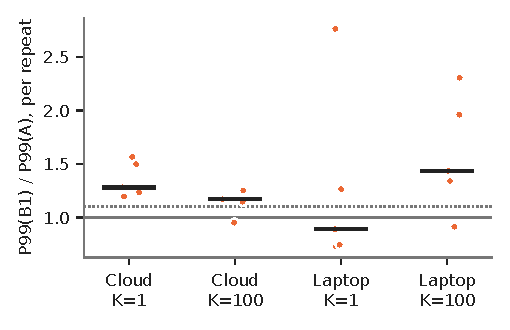
\includegraphics[width=\linewidth]{fig_ratio_two_env.pdf}
\caption{Per-repeat P99(B1)/P99(A) in the controlled replication (XGBoost, $W=30$, one inference thread, five repeats of 5,000 measured requests per path). Dots are repeats, bars medians; values above one favour A. The solid line marks one and the dotted line the pre-specified scope threshold of 1.10.}
\label{fig:ratio}
\end{figure}

\begin{table*}[pos=htbp]
\caption{Controlled replication (XGBoost, $W=30$). Median ratio: median over five repeats of the paired P99(B1)/P99(A). B2 CV: coefficient of variation of the five B2 P99 values. P50 and P99: mean over five repeats of the per-repeat quantile of 5,000 measured requests (warm-up excluded), in milliseconds, with the SD of the per-repeat P99 in parentheses.}\label{tab:replication}
\small\setlength{\tabcolsep}{4pt}
\begin{tabular*}{\tblwidth}{@{\extracolsep{\fill}}l r r r r rrr rrr@{}}
\toprule
 & & & & & \multicolumn{3}{c}{P50 (ms)} & \multicolumn{3}{c}{P99 (ms)} \\
\cmidrule(lr){6-8}\cmidrule(lr){9-11}
Environment & $K$ & Median ratio & Repeats $>1$ & B2 CV & A & B1 & B2 & A & B1 & B2 \\
\midrule
Cloud & 1 & 1.28 & 5/5 & 0.014 & 0.831 & 1.074 & 0.620 & 1.78 (0.15) & 2.42 (0.42) & 1.36 (0.02) \\
Laptop & 1 & 0.89 & 2/5 & 0.087 & 0.975 & 1.201 & 0.601 & 4.07 (1.76) & 4.52 (2.04) & 2.32 (0.20) \\
Cloud & 100 & 1.17 & 4/5 & 0.072 & 0.862 & 1.068 & 0.629 & 1.89 (0.20) & 2.16 (0.13) & 1.48 (0.11) \\
Laptop & 100 & 1.43 & 4/5 & 0.234 & 0.898 & 1.222 & 0.604 & 2.80 (0.55) & 4.27 (1.08) & 2.58 (0.60) \\
\bottomrule
\end{tabular*}
\end{table*}

Two observations qualify these results. First, the aggregation changes the impression: on the laptop at $K=1$, the mean of per-repeat P99 is lower for A (4.07 versus 4.52\,ms) although the median paired ratio is below one, because one repeat has a ratio of 2.76 while three are below one. We therefore report the repeat-level ratios rather than a single percentage. Second, median latency is more stable than the tail: as a descriptive observation that was not one of the pre-specified rules, B1/A P50 exceeds one in all 20 paired repeats (range 1.08--1.47), consistent with B1's additional read and decoding. The causes of tail variation (scheduling, garbage collection, Redis or model calls) were not decomposed, and the maintained direction at $K=100$ does not show that larger $K$ favours A. In these original cells, B2 has the lowest mean P50 and P99.

\paragraph{Client CPU restriction} A further pre-specified check in the cloud environment ($K=1$, $W=30$, XGBoost, five repeats) restricted the client process to one or two cores while leaving Redis unrestricted, with the prediction that the median ratio stays above one in both conditions. It did: the median B1/A P99 ratio was 1.27 with one core (four of five repeats above one) and 1.19 with two cores (three of five), with B2 CVs of 0.11 and 0.08 and B1/A P50 above one in all ten repeats. The reversals in individual repeats again show that the tail comparison is not stable at the repeat level (per-repeat values in Supplement~S4).

\subsection{RQ1: Breadth Across Model Families}
\label{subsec:rq1ext}
Table~\ref{tab:extension} and Fig.~\ref{fig:extension} report the Breadth Evaluation. In all four runs all 450,000 requests succeeded, and at all 150,000 paired request positions B1 and B2 returned the same label and the same Stage-2 decision as A; this is agreement between paths, not a check against ground truth. In all original-input runs, the Stage-2 rates of each model are identical, and those of XGBoost (37.4\% and 39.7\%) equal the replication's, which confirms that the same schedule was replayed.

The median result is the same in all four runs and for all three model families: B1/A P50 exceeds one in all 120 paired repeats (ranges 1.05--1.98 in the cloud container, 1.01--2.16 and 1.06--1.96 on the two laptop occasions, and 1.06--1.92 on the shared host). The tail result depends on the model, the environment and the occasion. In the cloud container, five of six cells pass the noise rule: XGBoost (medians 1.20 and 1.21, five of five repeats above one at both $K$, close to the replication's 1.28 and 1.17) and logistic regression at $K=100$ (1.49) favour A in every repeat, whereas random forest has medians of 1.04 and 0.94 and falls under the limited-benefit rule. On the laptop, the noise rule flags five of six cells on the first occasion and two of six on the second. Where the cells are not flagged on the second occasion, the medians favour A (logistic regression at $K=100$: 1.50; random forest at $K=1$: 1.15; XGBoost: 1.52 and 1.26), whereas the only unflagged cell of the first occasion, random forest at $K=1$, has a median of 1.01. For XGBoost at $K=1$, the laptop median was 0.89 in the replication, 1.12 (flagged) on the first breadth occasion and 1.52 on the second, so the single-stream tail direction on this machine is not stable across occasions. On the shared host, every median ratio exceeds one; random forest at $K=1$ is flagged as noisy and two further cells contain one reversed repeat each. B2's mean P99 is below A's in every original-input cell but not in two shared-host cells (random forest at $K=1$: 2.09 versus 2.05\,ms; XGBoost at $K=100$: 0.89 versus 0.86\,ms), which illustrates why B2 should not be read as a latency floor. Stage-2 rates on the November input (58--94\%) differ from the original series; they reflect the input, not a change in the benchmark. Per-repeat values are in Supplement~S4.

\begin{figure*}[pos=htbp]
\centering
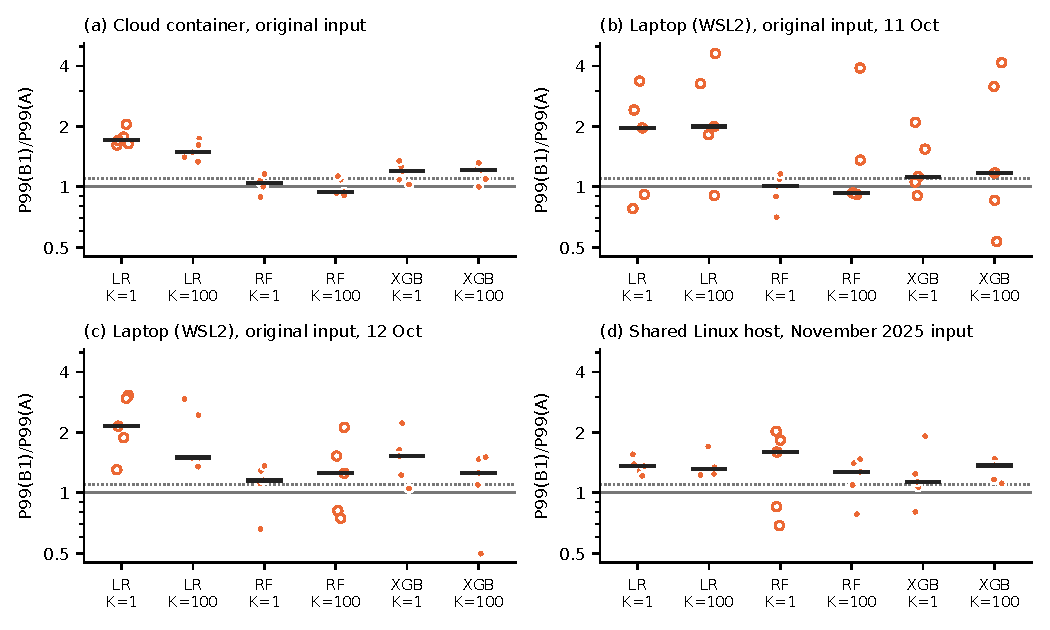
\includegraphics[width=0.9\linewidth]{fig_ratio_breadth.pdf}
\caption{Breadth Evaluation: per-repeat P99(B1)/P99(A) for the three model families ($W=30$, five repeats of 5,000 measured requests per path; logarithmic axis). (a)~New cloud container of the replication type and (b, c)~replication laptop on two occasions, all with the original input; (d)~shared Linux host with the November 2025 input. Bars mark medians; hollow markers denote cells flagged as noisy by the pre-specified B2 rule (CV $>0.25$), whose tail comparison is inconclusive. Lines as in Fig.~\ref{fig:ratio}.}
\label{fig:extension}
\end{figure*}

\begin{table*}[pos=htbp]
\caption{Breadth Evaluation. Each panel is one run and is not pooled with the other or with Table~\ref{tab:replication}. Columns as in Table~\ref{tab:replication}; P99 is the mean of five per-repeat P99 values in milliseconds. Stage-2: fraction of measured requests on which Stage~2 ran, identical for all paths and repeats of a cell. Status follows the pre-specified rules: noisy (B2 CV $>0.25$), limited (median ratio $\le1.10$), otherwise descriptive.}\label{tab:extension}
\small
\begin{tabular*}{\tblwidth}{@{\extracolsep{\fill}}l r r r r rrr r l@{}}
\toprule
 & & & & & \multicolumn{3}{c}{Mean P99 (ms)} & & \\
\cmidrule(lr){6-8}
Model & $K$ & Median ratio & Repeats $>1$ & B2 CV & A & B1 & B2 & Stage-2 & Status \\
\midrule
\multicolumn{10}{@{}l}{\emph{(a) Cloud container of the replication type, original input (2026-10-12)}} \\
Logistic & 1 & 1.71 & 5/5 & 0.360 & 0.879 & 1.533 & 0.472 & 26.2\% & noisy \\
Logistic & 100 & 1.49 & 5/5 & 0.077 & 0.854 & 1.280 & 0.444 & 28.8\% & descriptive \\
Random forest & 1 & 1.04 & 4/5 & 0.084 & 3.159 & 3.242 & 2.530 & 35.7\% & limited \\
Random forest & 100 & 0.94 & 2/5 & 0.092 & 3.376 & 3.343 & 2.569 & 40.3\% & limited \\
XGBoost & 1 & 1.20 & 5/5 & 0.062 & 1.961 & 2.315 & 1.485 & 37.4\% & descriptive \\
XGBoost & 100 & 1.21 & 5/5 & 0.093 & 1.975 & 2.302 & 1.597 & 39.7\% & descriptive \\
\midrule
\multicolumn{10}{@{}l}{\emph{(b) Replication laptop, original input, first occasion (2026-10-11)}} \\
Logistic & 1 & 1.97 & 3/5 & 0.287 & 1.610 & 2.507 & 0.664 & 26.2\% & noisy \\
Logistic & 100 & 1.99 & 4/5 & 0.337 & 1.497 & 3.415 & 0.667 & 28.8\% & noisy \\
Random forest & 1 & 1.01 & 3/5 & 0.211 & 6.525 & 6.242 & 3.761 & 35.7\% & limited \\
Random forest & 100 & 0.93 & 2/5 & 0.315 & 5.583 & 7.455 & 4.188 & 40.3\% & noisy \\
XGBoost & 1 & 1.12 & 4/5 & 0.377 & 3.831 & 4.861 & 2.718 & 37.4\% & noisy \\
XGBoost & 100 & 1.17 & 3/5 & 0.437 & 3.666 & 5.305 & 2.444 & 39.7\% & noisy \\
\midrule
\multicolumn{10}{@{}l}{\emph{(c) Replication laptop, original input, second occasion (2026-10-12)}} \\
Logistic & 1 & 2.15 & 5/5 & 0.279 & 1.514 & 3.353 & 0.694 & 26.2\% & noisy \\
Logistic & 100 & 1.50 & 5/5 & 0.121 & 1.565 & 2.938 & 0.794 & 28.8\% & descriptive \\
Random forest & 1 & 1.15 & 4/5 & 0.189 & 5.283 & 5.709 & 3.214 & 35.7\% & descriptive \\
Random forest & 100 & 1.25 & 3/5 & 0.353 & 4.885 & 5.801 & 4.775 & 40.3\% & noisy \\
XGBoost & 1 & 1.52 & 5/5 & 0.197 & 3.048 & 4.423 & 2.004 & 37.4\% & descriptive \\
XGBoost & 100 & 1.26 & 4/5 & 0.192 & 4.633 & 5.087 & 2.235 & 39.7\% & descriptive \\
\midrule
\multicolumn{10}{@{}l}{\emph{(d) Shared Linux host, November 2025 input (2026-10-11)}} \\
Logistic & 1 & 1.36 & 5/5 & 0.230 & 0.612 & 0.829 & 0.402 & 93.1\% & descriptive \\
Logistic & 100 & 1.32 & 5/5 & 0.212 & 0.600 & 0.810 & 0.436 & 94.0\% & descriptive \\
Random forest & 1 & 1.60 & 3/5 & 0.401 & 2.052 & 2.495 & 2.094 & 90.3\% & noisy \\
Random forest & 100 & 1.27 & 4/5 & 0.177 & 1.737 & 2.045 & 1.657 & 89.0\% & descriptive \\
XGBoost & 1 & 1.14 & 4/5 & 0.052 & 1.178 & 1.330 & 0.815 & 58.4\% & descriptive \\
XGBoost & 100 & 1.37 & 5/5 & 0.231 & 0.861 & 1.118 & 0.888 & 58.9\% & descriptive \\
\bottomrule
\end{tabular*}
\end{table*}

\paragraph{Answer to RQ1} Avoiding the window read lowered median per-request latency in every paired repeat of the replication and of all three breadth runs, for all three model families. The tail effect was smaller and depended on environment and model. With 100 resident streams it was maintained across the two replication environments, but with one stream it reversed on the laptop. In the breadth runs it favoured A for XGBoost and logistic regression wherever the noise rule did not flag the cell, was small and inconsistent for random forest (medians 0.94 to 1.15 where unflagged on the original input), was inconclusive in seven of twelve laptop cells over two occasions, and for XGBoost at $K=1$ on the laptop it changed between occasions (0.89, 1.12 and 1.52).

\subsection{RQ2: Mechanism}
\label{subsec:rq2}
\paragraph{Prediction equivalence} On the rule-selected windows, B1 and B2 produced the same label as A on every tick, for all three model families and in both environments (18,000 path-level records; 12,000 comparisons against A; zero mismatches). The windows start at rows 700, 0 and 0 for logistic regression, random forest and XGBoost; Stage~2 ran on 214, 224 and 307 of their 1,000 ticks and both Stage-2 labels occurred (73/141, 32/192 and 46/261 ticks with label 1/2). Table~\ref{tab:e0} gives the counts. Together with the identical writer and stored layout, this confirms that the A/B1 comparison varies only the state-access path. It does not compare probabilities, prove equivalence for all inputs, or measure accuracy.

\begin{table}[pos=htbp]
\caption{Prediction equivalence on rule-selected 1,000-row windows; identical in both environments. Start: first row; S2: ticks on which Stage~2 ran; 1/2: labels 1 and 2 among them; B1, B2: label mismatches against A.}\label{tab:e0}
\small
\begin{tabular*}{\tblwidth}{@{\extracolsep{\fill}}l r r r r r@{}}
\toprule
Model & Start & S2 & 1/2 & B1 & B2 \\
\midrule
Logistic & 700 & 214 & 73/141 & 0 & 0 \\
Rand.\ forest & 0 & 224 & 32/192 & 0 & 0 \\
XGBoost & 0 & 307 & 46/261 & 0 & 0 \\
\bottomrule
\end{tabular*}
\end{table}

\paragraph{State cost versus window length} Figure~\ref{fig:window} and Table~\ref{tab:window} show the window sweep. B1's mean state interval rises from 0.387\,ms at $W=10$ to 0.614\,ms at $W=120$ (+59\%), whereas A's stays between 0.214 and 0.233\,ms (+9\%; the ratio of maximum to minimum, 1.09, is within the pre-specified bound of 1.25). B2's local recomputation rises from 0.068 to 0.078\,ms. The B1/A P99 ratio exceeds one in all five repeats at every $W$, but its medians (1.30, 1.30, 1.14, 1.47) are not monotonic in $W$; the pre-specified descriptive prediction that the tail ratio increases with $W$ is met only in sign (Spearman $\rho=0.40$ over four values). The sweep therefore supports the access-cost mechanism, not a $W$-driven law for total tail latency; model execution and host variability may dilute the state-access difference at the tail, which was not isolated.

\begin{figure}[pos=htbp]
\centering
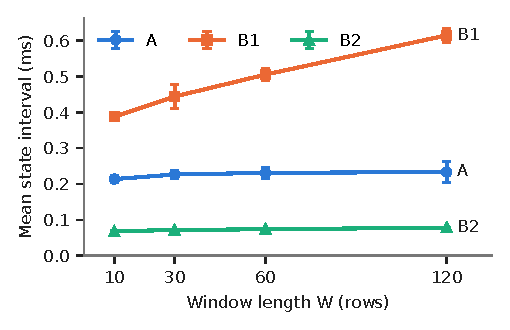
\includegraphics[width=\linewidth]{fig_state_vs_W.pdf}
\caption{Mean per-request state interval versus window length (cloud, $K=1$, XGBoost, one inference thread; mean $\pm$ SD over five repeats of 5,000 requests). A: Lua update; B1: same update plus window read and decoding; B2: local slice and recomputation.}
\label{fig:window}
\end{figure}

\begin{table}[pos=htbp]
\caption{Window sweep (cloud, $K=1$, XGBoost). State: mean over five repeats of the per-repeat mean state interval. P99: mean of per-repeat P99. Median ratio: median paired P99(B1)/P99(A). Milliseconds.}\label{tab:window}
\small
\begin{tabular*}{\tblwidth}{@{\extracolsep{\fill}}r rrr rr r@{}}
\toprule
 & \multicolumn{3}{c}{State} & \multicolumn{2}{c}{P99} & \\
\cmidrule(lr){2-4}\cmidrule(lr){5-6}
$W$ & A & B1 & B2 & A & B1 & Ratio \\
\midrule
10 & 0.214 & 0.387 & 0.068 & 1.540 & 1.932 & 1.30 \\
30 & 0.226 & 0.444 & 0.072 & 1.665 & 2.152 & 1.30 \\
60 & 0.231 & 0.505 & 0.074 & 1.729 & 2.192 & 1.14 \\
120 & 0.233 & 0.614 & 0.078 & 1.692 & 2.341 & 1.47 \\
\bottomrule
\end{tabular*}
\end{table}

\paragraph{Bounded state} For each $W$, Redis \texttt{MEMORY USAGE} of the window key was identical at every checkpoint from $N=W$ to $N=20{,}000$, with zero SD over five repeats, and the list length equalled $W$ (Fig.~\ref{fig:memory}). The footprint increases with $W$ alongside the logical payload $4dW$: 488, 1,064, 1,960 and 3,752 bytes for $W=10$, 30, 60 and 120, against 240, 720, 1,440 and 2,880 bytes of payload; the difference reflects per-entry, object and key-name overhead. Exact values depend on the key name, Redis build, encoding and allocator, and four values of $W$ do not establish an allocator law. A and B1 share this layout; across $K$ streams the window state is $K$ times the per-key footprint.

\begin{figure*}[pos=htbp]
\centering
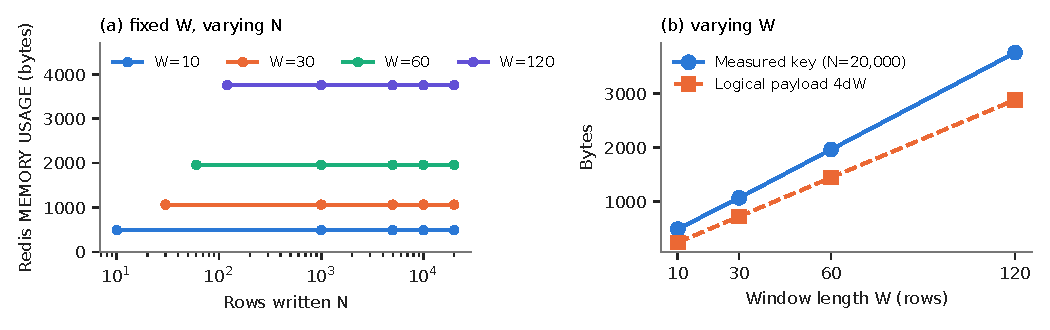
\includegraphics[width=0.9\linewidth]{fig_memory.pdf}
\caption{Redis key memory of the bounded window, measured without inference (five repeats; SD is zero at every point). (a)~For fixed $W$, \texttt{MEMORY USAGE} does not change with the number of rows written. (b)~At $N=20{,}000$, the footprint increases with $W$ alongside the logical float32 payload $4dW$ ($d=6$).}
\label{fig:memory}
\end{figure*}

\paragraph{Update methods} Sequential commands, the pipeline and the Lua script produced byte-identical final lists for all four $W$; after every update the length equalled $\min(t,W)$ and the head held the newest 24-byte vector. These checks cover a single sequential writer. Update-only latency (Table~\ref{tab:update}) is highest for the two-round-trip sequential method; the pipeline and Lua medians are close, and at P99 the variation between repeats exceeds the differences between methods (per-repeat values in Supplement~S3).

\begin{table}[pos=htbp]
\caption{Update-only latency in \emph{microseconds} (cloud, direct Redis 7.0.15 on loopback, $W=30$, $d=6$, no inference). Mean (SD) over five repeats of the per-repeat quantile of 2,000 measured updates.}\label{tab:update}
\small
\begin{tabular*}{\tblwidth}{@{\extracolsep{\fill}}l r r r@{}}
\toprule
Method & Round trips & P50 ($\mu$s) & P99 ($\mu$s) \\
\midrule
Sequential & 2 & 255 (35) & 1,828 (1,315) \\
Pipeline & 1 & 162 (19) & 1,606 (730) \\
Lua script & 1 & 138 (23) & 1,020 (968) \\
\bottomrule
\end{tabular*}
\end{table}

\paragraph{Answer to RQ2} Because A and B1 share writer, layout, model input and predictions, their difference is the window read and decoding, whose cost grows with $W$ while the update-only path stays nearly flat. The stored state is constant in $N$ for fixed $W$ and $d$ and increases with $W$ and $K$.

%% ==================================================================
\section{Discussion: Architectural Trade-offs (RQ3)}
\label{sec:discussion}
%% ==================================================================
\subsection{When External State Is Required}
In every replication cell and every original-input breadth cell, the in-process reference B2 had the lowest mean P50 and P99; on the shared host it had the lowest P50 but not always the lowest P99. When a single process can own ephemeral state and minimum latency is the only objective, local memory is the natural choice, and nothing in this paper argues otherwise. External state becomes relevant when other processes must read the state, when state must outlive the inference process, or when inference and storage are deployed and scaled separately. These are requirements of the surrounding system rather than properties of the latency measurements. Whether they are met depends on choices outside the decision path: Redis persistence (snapshots or an append-only log with a chosen fsync policy), replication and failover, a recovery protocol for the cold tier, and ordering or idempotency rules for writers. Our measurements cover the synchronous state-access path only; they do not establish crash durability, failover behaviour or concurrent-writer correctness, and the breadth runs used Redis with persistence disabled. If A's synchronous write fails, the current implementation does not reconstruct or fail over automatically. Table~\ref{tab:tradeoff} summarises how the three paths relate to these requirements and which relations this paper measured.

\begin{table*}[pos=htbp]
\caption{Requirements versus execution paths. ``Measured'' entries are supported by Section~\ref{sec:results}; the others are properties of the design or of Redis configuration that were not tested.}\label{tab:tradeoff}
\small
\begin{tabularx}{\linewidth}{@{}>{\raggedright\arraybackslash}p{0.2\linewidth} Y Y Y >{\raggedright\arraybackslash}p{0.15\linewidth}@{}}
\toprule
Requirement & A (DASH) & B1 (window fetch) & B2 (in-process) & Evidence here \\
\midrule
Low synchronous state-access cost & One Lua call; $\mathcal{O}(d)$ transfer & Lua call plus $\mathcal{O}(Wd)$ read and decode & No store access & Measured \\
State size independent of history & Window key constant in $N$ & Same key as A & Replay array (whole input in the benchmark) & Measured (A/B1 key) \\
State readable by other processes & Yes, Redis key & Yes, Redis key & No & Design property \\
State outlives the inference process & Kept by the Redis server & As A & Lost & Not tested \\
State survives a store failure & Depends on RDB/AOF and replication & As A & Not applicable & Not tested; persistence off in breadth runs \\
Several writers per stream & Per-list atomic update only; no cross-writer ordering & As A & Not applicable & Not tested \\
Recent history for non-model readers & Last $W$ vectors in Redis & Same & Local only & Design property \\
\bottomrule
\end{tabularx}
\end{table*}

\subsection{Latency Versus Operational Requirements}
Given that external state is required, the results show that the access discipline matters. A current-vector model does not need the window, so reading it back on every tick adds work proportional to $W$ to the decision path without changing the prediction. Removing that read lowered median latency in every paired repeat we measured. The tail is a different matter: its size and even its sign depended on the environment and on $K$, so a deployment that cares about P99 should measure the effect on its own host and store rather than assume it. The window itself is still kept in DASH. Its purpose is to provide recent history to readers other than the current-vector model (inspection, debugging, consumers that need context) and, in this study, to keep the stored layout identical across A and B1. If no such reader exists, a deployment could store only the recursive state and avoid the $\mathcal{O}(Wd)$ footprint as well; that variant was not evaluated. The cost that DASH removes is the unneeded \emph{read}, not the stored window.

Two further trade-offs follow from the design. The atomic Lua update protects a single list from interleaved push and trim, but a multi-step update across keys, or several writers to one stream, would need additional coordination. Conditional Stage-2 inference reduces how often the heavier model runs, but its effect depends on the data: the measured Stage-2 rate was 37--40\% on the original series and 58--94\% on the November 2025 archive under the same thresholds. Systems evaluations of gated models should therefore report the gate rate alongside latency.

\subsection{Design Guidelines}
Three guidelines for practitioners follow from the evidence, each limited by the threats in Section~\ref{sec:threats}. First, match the synchronous read to what the model consumes: a current-vector model should receive the current vector, and history should be read only by the components that need it. Second, evaluate an external-state design against an in-process reference on the same host and schedule, so that the price of externalisation is visible, and report per-repeat tail values rather than a single pooled percentile. Third, specify the operational properties that justify external state (persistence mode, recovery procedure, writer model) together with the latency results, because they are configured separately and are not implied by the presence of a Redis key.

\subsection{Transferability}
The argument applies to streaming workloads whose features admit fixed-size recursive updates and whose model consumes a fixed-width current representation, such as fraud screening or telemetry monitoring. It does not apply to sequence models that need the window as input; for them the read is necessary. The magnitude of the benefit depends on the cost of the read relative to model execution: in all three breadth runs, the mean P50 ratio B1/A was largest for logistic regression, the cheapest model (1.54--1.89), and smallest for random forest, the most expensive (1.18--1.23). At the tail, random forest's unflagged P99 ratios on the original input ranged from 0.94 to 1.15 (cloud container 1.04 and 0.94; laptop 1.01 and 1.15 on the two occasions): when model execution dominates the tail, removing the read changes it little. The measurements were made with Redis on the same host as the client, so a network-separated store, where the read also crosses a network, remains to be measured.

%% ==================================================================
\section{Threats to Validity}
\label{sec:threats}
%% ==================================================================
\paragraph{Internal validity} The two replication environments differ in processor, virtualisation, operating-system layer and Redis version at once, so a disagreement between them cannot be attributed to one factor. Path order was randomised with a seed and inference was pinned to one thread, but host jitter remains: the driver also runs a light background CPU-sampling thread during measurement, and the November 2025 breadth run used a host shared with other work. The schedule and stream segmentation change with $K$. The models, scaler and thresholds are fixed artefacts whose training run was reconstructed after the fact (Section~\ref{subsec:artefacts}); the reconstruction reproduces the scaler and all stored thresholds, but the run's console output was not archived. The threshold routine's indexing defect has a negligible effect on the stored operating points, and the archived ``test'' metrics overlap the validation set. These issues affect the predictive interpretation of the workload, not the paired systems comparison, because all paths use the same artefacts. The earlier evaluation of a previous implementation lacks matching trial-level provenance and is not used as evidence.

\paragraph{Construct validity} Latency is measured inside the per-request function and excludes ingestion, binning, feature generation, cold-tier writes and alert delivery, so it is not a service-level latency. $K$ counts replicated resident streams served by one closed-loop client, not concurrent load or distinct assets. Key memory is the Redis \texttt{MEMORY USAGE} of one window key, not process RSS or total application memory. Prediction equivalence is label agreement on selected windows, not accuracy. B2's recomputation is synthetic window work whose result is discarded. Durability, recoverability and shared access motivate the design but were not measured.

\paragraph{External validity} Redis ran locally in every environment; there is no network-separated store, multi-writer or failover experiment and no comparison with managed-state stream processors. XGBoost latency was measured in both replication environments; logistic-regression and random-forest latency were measured with the original input on the replication laptop and in a new cloud container of the replication type (not the same instance), and on a third host with a different input; equivalence was checked for all three families in both replication environments. The workload is one asset and one feature set, and the equivalence windows were selected to exercise Stage~2.

\paragraph{Conclusion validity} Each cell has five repeats, and requests within a repeat are serially dependent, so the results are descriptive and no significance or equivalence test is claimed beyond the observed label matches. P99 values rest on about 50 observations per repeat, and reversals occur in individual repeats. The B2 noise rule (CV $>0.25$) flagged one cloud breadth cell, one shared-host cell and seven of twelve laptop breadth cells over two occasions, which are reported as inconclusive, and several further cells (laptop $K=100$ in the replication; shared-host logistic regression at both $K$ and XGBoost at $K=100$; laptop random forest at $K=1$) lie between 0.21 and 0.24, close to the threshold; the rules were pre-specified but not externally registered.

%% ==================================================================
\section{Conclusion}
\label{sec:conclusion}
%% ==================================================================
When a streaming ML service must keep per-stream state outside the inference process, the way that state is accessed becomes part of the latency budget. DASH maintains a bounded window with a single atomic update and gives current-vector models the current vector without reading the window back. In a controlled two-environment replication in which the compared paths share writer, stored layout, models and schedule and agree on every predicted label tested, the window-fetching path's state cost grew with $W$ while the bounded path's stayed nearly flat, the Redis key footprint was constant in $N$ for a fixed $W$ and $d$, and median latency was lower without the read in every paired repeat.

The tail-latency benefit is narrower. The P99 direction was maintained across environments with 100 resident streams but reversed on one environment with a single stream, A breadth evaluation with all three model families confirmed the median-latency reduction in both environment types and on a third host; tail gains held for logistic regression and XGBoost where measurements were not noisy, but were small and inconsistent for random forest, whose inference dominates the tail, and laptop tails varied between occasions. The in-process reference was faster in all replication cells, but not in every breadth cell, and is not an absolute bound.

DASH is therefore a design rule for the case in which external state is required, not a claim that external state beats local memory or that tail latency always improves. Network-separated stores, concurrent writers, measured recovery and comparison with managed-state backends are the next steps.

%% ------------------------------------------------------------------
\printcredits

\section*{Declaration of competing interest}
The authors declare that they have no known competing financial interests or personal relationships that could have appeared to influence the work reported in this paper.

\section*{Funding}
This research did not receive any specific grant from funding agencies in the public, commercial, or not-for-profit sectors.

\section*{Declaration of generative AI and AI-assisted technologies in the manuscript preparation process}
During the preparation of this work the authors used Claude (Anthropic) and ChatGPT (OpenAI) to assist with experiment scripting, re-analysis and auditing of archived experiment records, and language editing; the cloud-container breadth run (Section~\ref{subsec:extension_design}) was executed by the AI assistant in its sandbox environment from the authors' input files and frozen code. After using these tools, the authors reviewed and edited the content as needed and take full responsibility for the content of the published article.

\section*{Data availability}
The implementation, frozen model artefacts, thresholds, and the controlled-replication scripts, per-request outputs, environment metadata and SHA-256 input manifests are available at \url{https://github.com/swk99/dash-bound-state} (commit \texttt{5335376}, directory \texttt{experiments/2026-10-02/}; the full commit hash and all file hashes are listed in Supplement~S7). The 75 input feature files of the controlled replication are not in the repository; their hashes are recorded in its manifest. Exact regeneration of these features from public Binance archives (\url{https://data.binance.vision}) would additionally require the original archive files, conversion command, chunk boundaries and initial states, which are not all documented. The analysis scripts used in this revision to recompute every reported quantity from the per-request records, the raw records and metadata of both breadth runs, and the file manifest of the November 2025 input archive are provided with the supplementary material.

%% ==================================================================
\bibliographystyle{cas-model2-names}
\bibliography{references}

\end{document}
